%! TEX root = diss.tex
\documentclass[../diss.tex]{subfiles}

\appendix

\chapter{Further definitions}%
\label{cha:Further definitions}

\section{Abstract algebra}%
\label{sec:Abstract algebra}


\chapter{Proof of some theorem}

\section{Proof of that theorem}

It's a tautology obviously.

% Error bars {{{
\section{Error bars}%
\label{sec:Error bars}

Behold, the plots with error bars:

% Sandy bridge
\begin{figure}
    \begin{center}
        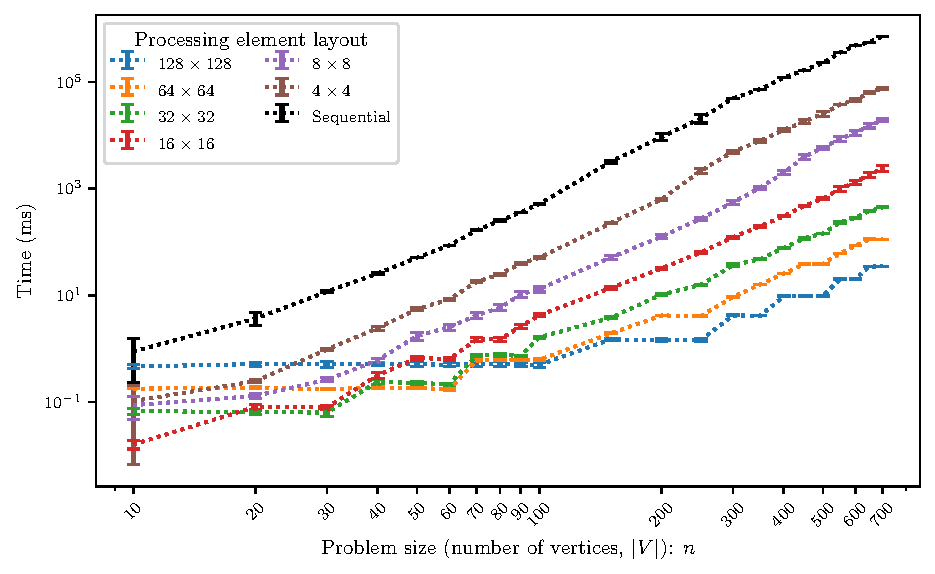
\includegraphics{figs/plots/total-time-scaling-sandy-full-width.pdf}
    \end{center}
    \caption{Sandy bridge total time scaling}
    \label{fig:appendix-plot-sandy-bridge}
\end{figure}

% Taihu light
\begin{figure}
    \begin{center}
        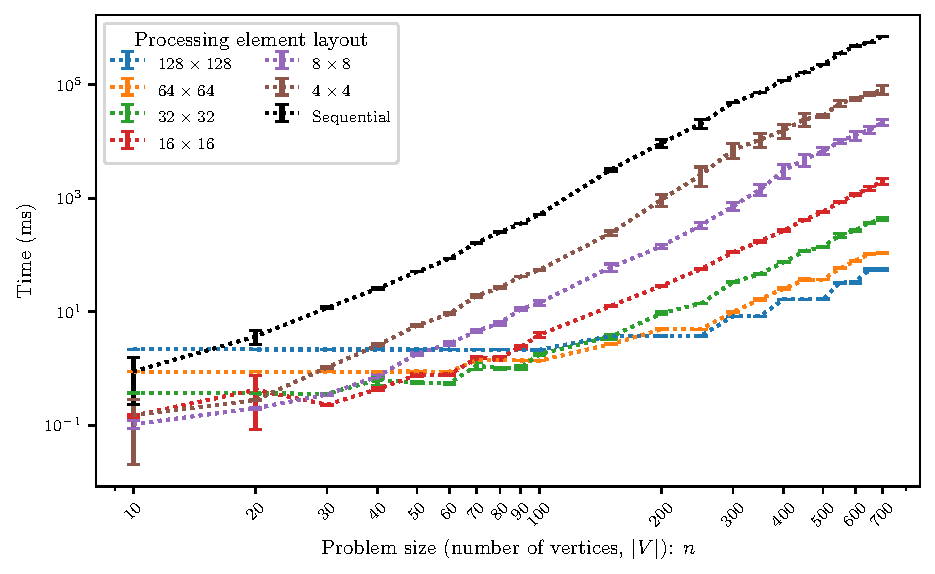
\includegraphics{figs/plots/total-time-scaling-taihu-full-width.pdf}
    \end{center}
    \caption{Taihu-Light total time scaling}
    \label{fig:appendix-plot-taihu-light}
\end{figure}

% Internet
\begin{figure}
    \begin{center}
        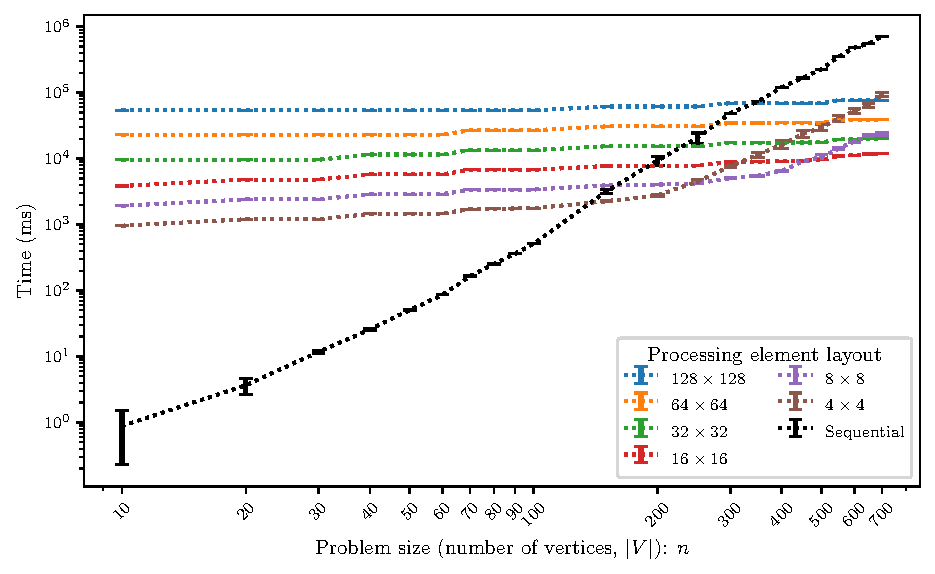
\includegraphics{figs/plots/total-time-scaling-internet-full-width.pdf}
    \end{center}
    \caption{Internet total time scaling}
    \label{fig:appendix-plot-internet}
\end{figure}

% }}}


% Project proposal
\chapter{Project Proposal}

% \subfile{../project-proposal/proposal}
